\chapter{Introduction}\label{ch:introduction}


\section{Artificial intelligence}

\newglossaryentry{ai}{name={AI},description={Artificial intelligence}}

A growing number of digital devices and the amount of information they produce and store has put Artificial intelligence (\gls{ai}) at the frontier of today's society.
AI has changed the perspective on such massive amounts of data, which are nowadays transformed from a mare record of an event to a carrier of useful information.
In a sense similar to the tests designed by psychologists and sociologists, AI allows us to sort through the mountains of data and exploit it to gain insights in many aspects of everyday life.
This potential is perhaps best summarised in a quote by the mathematician Clive Humbly:
\begin{quote}
	Data is the new oil. It’s valuable, but if unrefined it cannot really be used. It has to be changed into gas, plastic, chemicals, etc to create a valuable entity that drives profitable activity; so must data be broken down, analysed for it to have value.
\end{quote}
The exploitation of information has already significantly changed the landscape of todays economy over several past decades, most evident in the shift in the Forbes' \textit{Fortune 500} list.
This list, ranking the most successful companies worldwide, has traditionally been dominated by big oil companies.
However, in recent years IT companies have started to take over the dominion; among the ten most valuable companies, five are IT companies -- Apple, Alphabet, Microsoft, Amazon and Facebook.
Though AI is the core business only of Facebook and Alphabet's subsidiary Google, it plays a major role in business of the other companies.



% TODO: Despite the importance it is difficult to say What AI does - behaves intelligently
Despite its importance, it is still difficult to say what \gls{ai} precisely is.




Ai is a broad field including many different subfields and tasks, not all of them concerned with extracting insights from data.
Examples include problems of planning and scheduling, automated reasoning, theorem proving, robotics, language understanding and many others.
Many problems within AI often require a combination of different methods.
Last decades have also witnessed many breakthrough application of AI including AlphaGo \cite{SilverHuangEtAl16nature,silver2017mastering} which has dominated the best human player in the game of Go, Watson \cite{journals/aim/FerrucciBCFGKLMNPSW10} which has defeated the top human players in the question-answering game of Jeopardy!, self-driving cars and DeepBlue \cite{Hsu:2002:BDB:601291}  which defeated the world champion in chess, Gary Kasparov.





\section{Machine learning and logic}

\newglossaryentry{ml}{name={ML},description={Machine Learning}}
\newglossaryentry{srl}{name={SRL},description={Statistical relational learning}}
This thesis is situated in the subfields of AI called \textit{machine learning} (\gls{ml}) and \textit{statistical relational learning} (\gls{srl}).


Machine learning is probably the most prominent field of AI in the 21$^{\text{st}}$ century.
It concerns development of AI systems that \textit{improve their performance with experience}.
These systems learn concepts and skills from examples, provided by the expert, or through interaction with the environment, opening a possibility of new discovering knowledge.
Moreover, it brings the power of computer programming to non-experts, which could now program computer by simply providing examples of the desired task.



A common principle of many machine learning algorithms is that of learning a \textit{model of the world}. 
This assumes that a learning task is defined as a system with clearly defined inputs and outputs.
A typical machine learning algorithm is given the data, inputs and desired outputs, and its task is to discover a \textit{decision function}, system's gear wheels transforming the inputs to the output(s).
A huge variety of the existing machine learning algorithms differs in how they \textit{represent} the task.


% TODO: introduce an example that covers several ways of representing the decision function

\paragraph{Example (The art of machine learning in a nutshell)} Imagine your self choosing a new pet.
Being an \gls{ai} enthusiast, and having to choose among a vast variety of potential pets, you decide to use a machine learning algorithm to help you with the decision.
The first challenge you are faced with  is getting the data.
You decide to compile a large database of potential pets and identify their \textit{features} -- for example, the number of legs, level of fluffiness of their fur, their diary, whether they are playful of not, and whether they spit or bite.
These features define the \textit{inputs} for a machine learning algorithm.
We still have to provide the \textit{experience} to the learning algorithm in form of the desired outputs, which define the learning task.
The desired output come from the previous pets you owned and whether you liked having them as pets or not -- for example, imagine you have own a dog and a cat which you liked, and a duck which you were not so fond of.
These examples constitute our \textit{training data}, and are compiler in a simple Excel sheet (Table \ref{tab:pets}).



Once the data is compiled, you can proceed with learning the decision function mapping the inputs to the outputs.
This faces you with the second choice -- how should the decision function look like?
The straightforward choice seems to be a form of \texttt{IF-THEN} rules:
\begin{center}
	\texttt{IF} legs $=$ 4 \texttt{AND} fluffiness $\geq 4$ \texttt{THEN} yes.
\end{center}
An alternative option would be to assign an \textit{importance} to each feature so that a desirable potential pet gets a positive score, while the un-desirable one gets a negative score:

$$ w_1 \cdot \text{legs} + w_2 \cdot \text{fluffiness} + w_3 \cdot \text{diary} + w_4 \cdot \text{playful} - w_5 \cdot \text{spits} - w_6 \cdot \text{bites} - w_7 \geq 0$$

In this case, we would have to replace categorical choices, such as \texttt{playful} feature, with a numerical equivalent.
For example, we could replace \texttt{no} with 0, \texttt{sometimes} with 1 and \texttt{yes} with 2.
Many choices are possible, and the right one depends on the task at hand.



As the example X shows, it is necessary to differentiate between the representation of \textit{data} and the representation of  \textit{decision function}.
This thesis focuses on the data representation aspect and inherits the representation of decision function from the existing methods.

\begin{table}
	\centering
	\caption{Example dataset}
	\begin{tabular}{@{}lccccccc@{}}
		\toprule
		\textbf{ID} &\multicolumn{6}{c}{\textbf{Features}} 									& \textbf{Target} \\
		\cmidrule(lr){2-7} 
					& legs	& fluffiness		& diary 		& playful	& spits? 	& bites? 	&	\\
		\midrule
		cat			& 4		& 4				& carnivore	& sometimes & no		 	& sometimes	&  \checkmark \\
		dog			& 4		& 5				& carnivore	& yes		& no		& no		& \checkmark \\
		duck		& 2		& 2				& herbivore	& no			& no		& no		& $\times$ \\
		\multicolumn{8}{c}{\ldots} \\
		alpaca		& 4		& 5				& herbivore & yes		& sometimes	& no		& ? \\
		\bottomrule
	\end{tabular}
	\label{tab:pets}
\end{table}



The choice of data representation involves two issues.
First, one has to decide about the data representation \textit{format}.
Data format describe the basic form, a template, the data will take.
By far the most popular choice is the \textit{tabular representation}, e.g., Excel sheets, but other options include graphs, networks and even programming languages.
The second issue is concerned with the \textit{content} of the data itself, i.e., defining the \textit{features} of the task.
This populates the content of the specified template.



Both data representation aspects have a critical impact on the success of the machine learning application.
Choosing an insufficient data format prevents us from even capturing all intricacies of the data.
While tabular data format is by far the most popular one, it is also the least expressive one (it can capture only a simple data).
For example, complex graph structured data is impossible to represent in a simple Excel sheet.



A powerful way to overcome this representational limitations is to use \textit{predicate logic} as a data representation format. 
The field of AI combining machine learning with logic is known as \textit{Statistical relational Artificial intelligence} \cite{GetoorSRL,Raedt:2016:SRA:3027718} and Inductive logic programming \cite{LucRLbook}.
These methods combine three pillars of Artificial intelligence: it uses \textit{predicate logic} to represent complex data formats, \textit{probability theory} to capture the uncertainty of reasoning and \textit{machine learning} for learning models that leverage both logic and probability from data.
This renders SRL methods amongst the most expressive AI methods, i.e., they can easily represent tabular data, networks and graphs as well as entire computer programs. 



Selecting the appropriate format is rarely sufficient for a good performance -- choosing the right and informative features is the last step to cross.
Knowing which features carry the right information to solve the learning task is difficult, finding them requires an extensive domain knowledge. 
Consequently, finding informative features is typically a labour-intensive task, taking the vast majority of development of the machine learning model [citation?].



Motivated by the difficulty of manually finding informative features, machine learning practitioners have started to develop formal framework that can find informative features without expert intervention.
These methods fall under umbrella of \textit{representation} or \textit{deep learning} \cite{Goodfellow2016, Bengio:2009}.
\textit{Deep} refers to the idea of creating several layers of \textit{latent features} before solving the given task.
These methods, typically based on Artificial neural networks, have sparked a revolution within Artificial intelligence over the last decade.
As a result, many solution in the fields of computer vision, speech recognition and text processing have witnessed impressive improvements.
% TODO: put some of the results










\section{Motivations and Problem statement}

It is well known is psychology that the the ability of solving the task substantially depends on the way the task is represented.

% TODO: example arabic vs roman numbers addition; connect to 
\paragraph{Example} Consider the tasks in the Figure \ref{fig:cogease}.
The figure gives two simple addition tasks: one with arabic and the second one with roman numbers.
Both task are surely sufficiently easy to solve. 
However, paying attention to the effort it takes to solve each of the task, you will notice that solving the task on the right require more effort.
Moreover, it will take you more time solve it than the task on left.
Psychologists call this \textit{cognitive bias} [citation Kahneman and Tversky]; a measure of how easy it is for out brains to process information.
The state of cognitive ease is activated by confrontation with familiar concepts which do not require a significant effort.
The arabic system is the system we are confronted by every day and it, thus, does not require any extensive processing effort.
In contrast, the roman system is the one we are rarely confronted with after the primary school education and thus require a switch -- we are likely to solve it by \textit{mapping} the numbers to the arabic system.


 


\begin{figure}
	\centering
	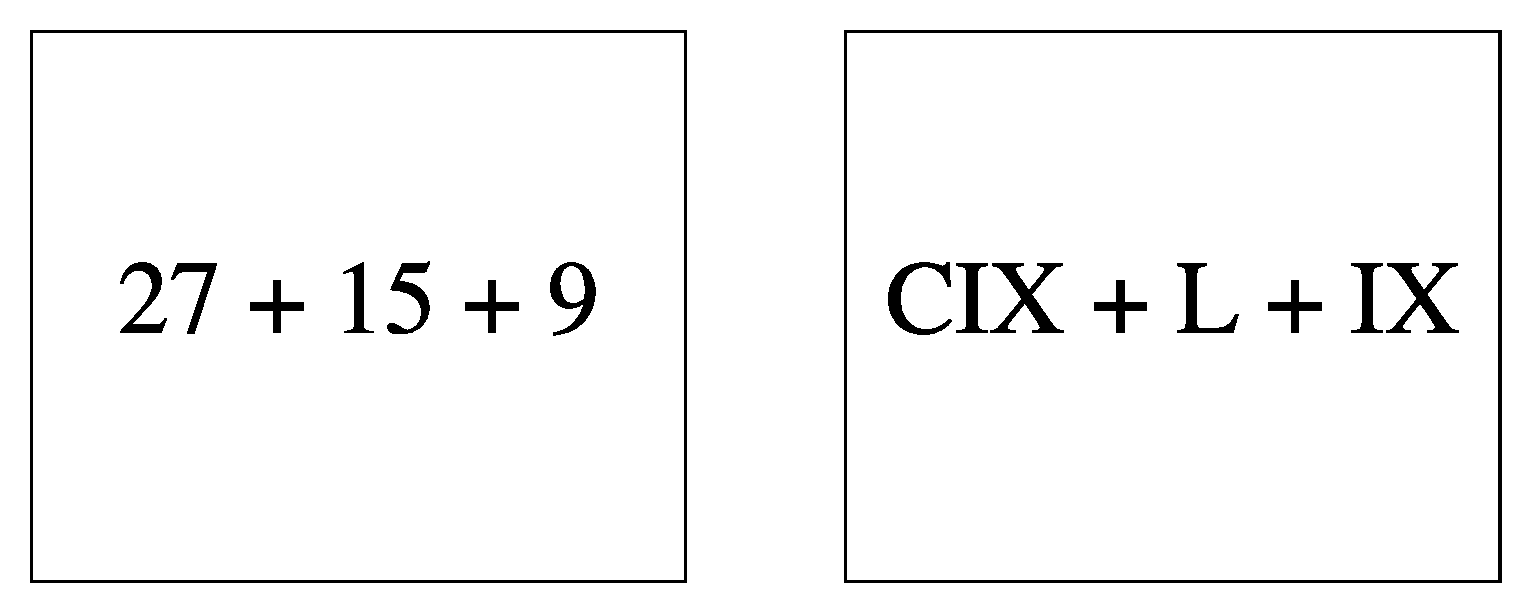
\includegraphics[width=\textwidth]{cognitiveEase}
	\caption{Cognitive ease}
	\label{fig:cogease}
\end{figure}

% TODO: give a simple algorithms exercise: searching for something in a set vs array


\paragraph{Example} Consider now a typical programming task from a first-year programming course: \textit{given a collection of elements, implement a function that checks whether a given element is present in the collection}.
If the collection of elements is small, the choice of the data structure representing the collection does not matter much.
However, if the collection of elements is large, for example containing tens of millions of elements, whether a set of an array is used as a data structure makes a large influence.
Using the sets one can check the existence of the elements almost instantly; in contrast, searching through an array resulting in traversing the collection until we find the required element.


% TODO: give an example of counting itemsets with a complex rules which elements should be counted 

\textbf{TODO: give an example of counting itemsets with a complex rule which elements should be counted; then  }


All of the examples above point to the same conclusion -- \textit{representation matters} both for human and computational problem solvers.
There is, therefore, a little surprise that one of the big revolutions in AI came from learning how to represent a given problem.



However, critically accessing the current progress of representation learning methods reveals several weaknesses.
First, the existing approaches extensively focus on tabular and signal-like data, such as images, speech and text.
Structured data, such as graphs and relational data, have only recently started to receive attention.
Moreover, the existing approaches for representation learning with relational data focuses on inventing new ways of re-representing relational data in a tabular format.
Second, the strong suit of logic based approaches to machine learning, besides their expressiveness, is their interpretability.
Currently the main tool for learning representations are Artificial neural networks, which are black-box models that are very difficult, if not impossible, to interpret.
Third, learning representations with neural networks is \textit{black magic}.
They are universal approximators, meaning they can approximate any function, but a lot of time is spent on finding the right architecture.
ANNS are ill fitted for structured problems. (Add )



% TODO: SRL methods have rich formalism for expressive complex problems and inference, but the learning is still difficult; therefore, RL can be helpful to simplify the learning


This thesis addresses the issues/limitation outline above.
It takes the opposite direction than the existing literature on representation learning with relational data: instead of approximating the more expressive logic framework with less expressive tabular format, we will lift the ideas from the representation learning to logical framework.
This view offers several benefits.
First, it is very expressive as it uses the programming language to define the decision functions.
Second, it is declarative.
Third, it is interpretable.



Our long term goal is to develop the tools that allow the methods from artificial intelligence and machine learning to 







% TODO: long term objective - SRL systems that can change the representation of the task that suits them the best



\section{Thesis contributions}

In this thesis we focus on the following research question:

\begin{quote}
	How can we lift the existing representation learning techniques to the rich knowledge representation framework of predicate logic?
\end{quote}


We identify \textit{four main contributions} within this thesis addressing that research question.



\subsubsection{A versatile relational clustering framework}

The first main contribution of the thesis is a new \textit{versatile relational clustering method}.
The proposed clustering framework consists of a novel similarity measure for both objects and relationships in relational data.
The main novelty of the proposed framework is that it comprises several \textit{interpretations of similarity} of relational data, e.g. similarity in terms of attributes or structures of the neighbourhood, in contrast to the existing methods in the literature which typically impose a very strict bias on what the similarity means.
The introduced framework specified only the similarity measure and, therefore, can be further combined with any clustering algorithm.




\subsubsection{Learning latent features by detecting approximate symmetries}

The second main contribution of the thesis is a framework for learning relational latent feature by detecting \textit{approximate symmetries} in data, termed CUR$^2$LED.
This approach is rooted in the idea that identifying similar objects in data, and finding what makes them similar, is a useful proxy towards identifying good features.
To identify the symmetries in objects and their relationships, this approach relies on the previously proposed relational clustering methods.
As knowing which kind of symmetries would be useful for a task is very difficult, if not impossible, the proposed approach makes use of many kinds of symmetries exploiting the previously introduced notion of interpretation of similarity.
 






\subsubsection{Auto-encoding logic programs}

The third main contribution of the thesis are \textit{auto-encoding logic programs} -- a logical generalisation of auto-encoders.
Auto-encoders are among the most versatile representation learning components applicable to many different learning settings.
This versatility makes them very suitable to the variety of SRL learning tasks, such as generative modelling and supervised learning, as the same latent representation can be re-use in many tasks.
We introduce a declarative framework for learning relational auto-encoders which are implemented as logic programs, instead of matrix computation as with more standard auto-encoders.






\subsubsection{Analysis of relational representation learning approaches}

The fourth contribution of this thesis is the empirical analysis and comparison of several relational representation learning methods.
First, we focus on better understanding CUR$^2$LED and show that the created latent features match well with the existing labels, which explains why such latent features are beneficial.
Second, we compare symbolic relational learning approaches to the prototypical \textit{knowledge graph embedding methods} -- a novel paradigm for relational learning rooted in representation learning, which approaches the problem by mapping logical symbols to points in Euclidean space.
We compare their performance on various relational dataset, identify their strengths and weaknesses and show that a good idea might be a hybrid learner exploit the strengths of both sides.




% TODO: contribution 5 - hybrid learner




\section{Structure of the thesis}


The work in this theses combines the fields of \textit{statistical relational learning} and \textit{representation learning}.
We review the basic foundations Statistical Relational learning in \textbf{Chapter \ref{ch:learninglogic}} and Representation learning in \textbf{Chapter \ref{ch:learningrepresentations}}.


\textbf{Chapter \ref{ch:clustering}} presents a versatile clustering framework for relational data.
The key contributions of this chapter are (i) a novel similarity measure for relational objects, based on the summarisation of neighbourhood of individual objects, and (ii) a general framework for clustering both objects and relationships in the data.
The major novelty of the proposed framework is that it relies on several ways to define a similarity, instead of using only one way to look at it.
This chapter is based on the following publications:

\begin{quote}
	\bibentry{Dumancic2017a}
\end{quote}

\begin{quote}
	\bibentry{Dumancic2017}
\end{quote}



The following chapters explore different ideas towards learning relational latent features.
\textbf{Chapter \ref{ch:symmetries}} introduces the idea of using approximate symmetries in data as a latent representation of data.
It relies on the previously introduced relational clustering framework to identify various approximate symmetries, i.e. groups of relational objects that are \textit{similar} but not \textit{identical} to each other, and treats the identified symmetries as latent features.
\textbf{Chapter \ref{ch:alps}} introduces \textit{auto-encoding logic programs}, a declarative generalisation of the auto-encoder architecture \cite{Hinton504} that uses logic programs as a computational framework.
It introduces a general modelling framework for auto-encoding logic programs, as well as a general solver based on the constraint satisfaction problem that learns them from the declarative models provided by the user.
These chapters are based on the following publications:

\begin{quote}
	\bibentry{Dumancic2017}
\end{quote}

\begin{quote}
	\bibentry{Dumancic2017b}
\end{quote}

\begin{quote}
	\bibentry{Dumancic2018a}
\end{quote}


\textbf{Chapter \ref{ch:embeddinganalysis}} summarises the insights found by comparing various relational representation learning methods.
The analysis focuses on identifying strengths and weaknesses of various methods, as well as conditions under which different methods are applicable.
This chapter is based on the following publications

\begin{quote}
	\bibentry{Dumancic2017b}
\end{quote}

\begin{quote}
	\bibentry{Dumancic2018}
\end{quote}


The final chapter summarises the thesis, discusses its implications and provides a look into directions for \textit{future work}.







%%%%%%%%%%%%%%%%%%%%%%%%%%%%%%%%%%%%%%%%%%%%%%%%%%
% Keep the following \cleardoublepage at the end of this file, 
% otherwise \includeonly includes empty pages.
\cleardoublepage

% vim: tw=70 nocindent expandtab foldmethod=marker foldmarker={{{}{,}{}}}
 